\begin{table}
	\caption{Files provided by kaggle}
	\label{table:dataset-files}
	\begin{tabular}{ l | l }
		\hline
		File name & Format \\ \hline
		sample\_submission.csv & .zip (49.44 kb) \\
		train.csv & .zip (24.12 kb) \\
		imgs & .zip (8.73 gb) \\
		w\_7489 & .zip (710.90 kb) \\
		imgs\_subset & .zip (398.08 mb) \\
	\end{tabular}
\end{table}

The dataset is given through the competition from the kaggle website. Table \ref{table:dataset-files} shows the files and format of provided files data. The total size of the dataset is ~9 gb with 11468 different images which varies in dimension from 1000x1500px to 4000x6000px they do however all have the ratio of 1/5.

\begin{itemize}
	\item \emph{imgs.zip} contain all the images for both training and testing.
	\item \emph{train.csv} contains information about what whale is in what picture, in the format of image name and whale id.
	\item \emph{sample\_submission.csv} is en example of what a submission should look like.
	\item \emph{imgs\_subset.zip} is a subset of the images, containing the first 500 images.
	\item \emph{w\-7489.zip} contains a single image from the total set of images.
\end{itemize}

The training data contains information of 4544 different images, and 447 different whales, these labeled images are those being used for this project. The pictures are taken from above and Figure \ref{fig:whale-example} shows the content of the 'w\_7489.zip' file, which is a good example of the general content of the images look. The images can have whales facing any direction, placed anywhere and having none to all of its 'face' visible, they can also contain splashes from waves, other whales or the whale itself. Some images have multiple whales and some show the tails of other whales.

\begin{figure}
	\centering
	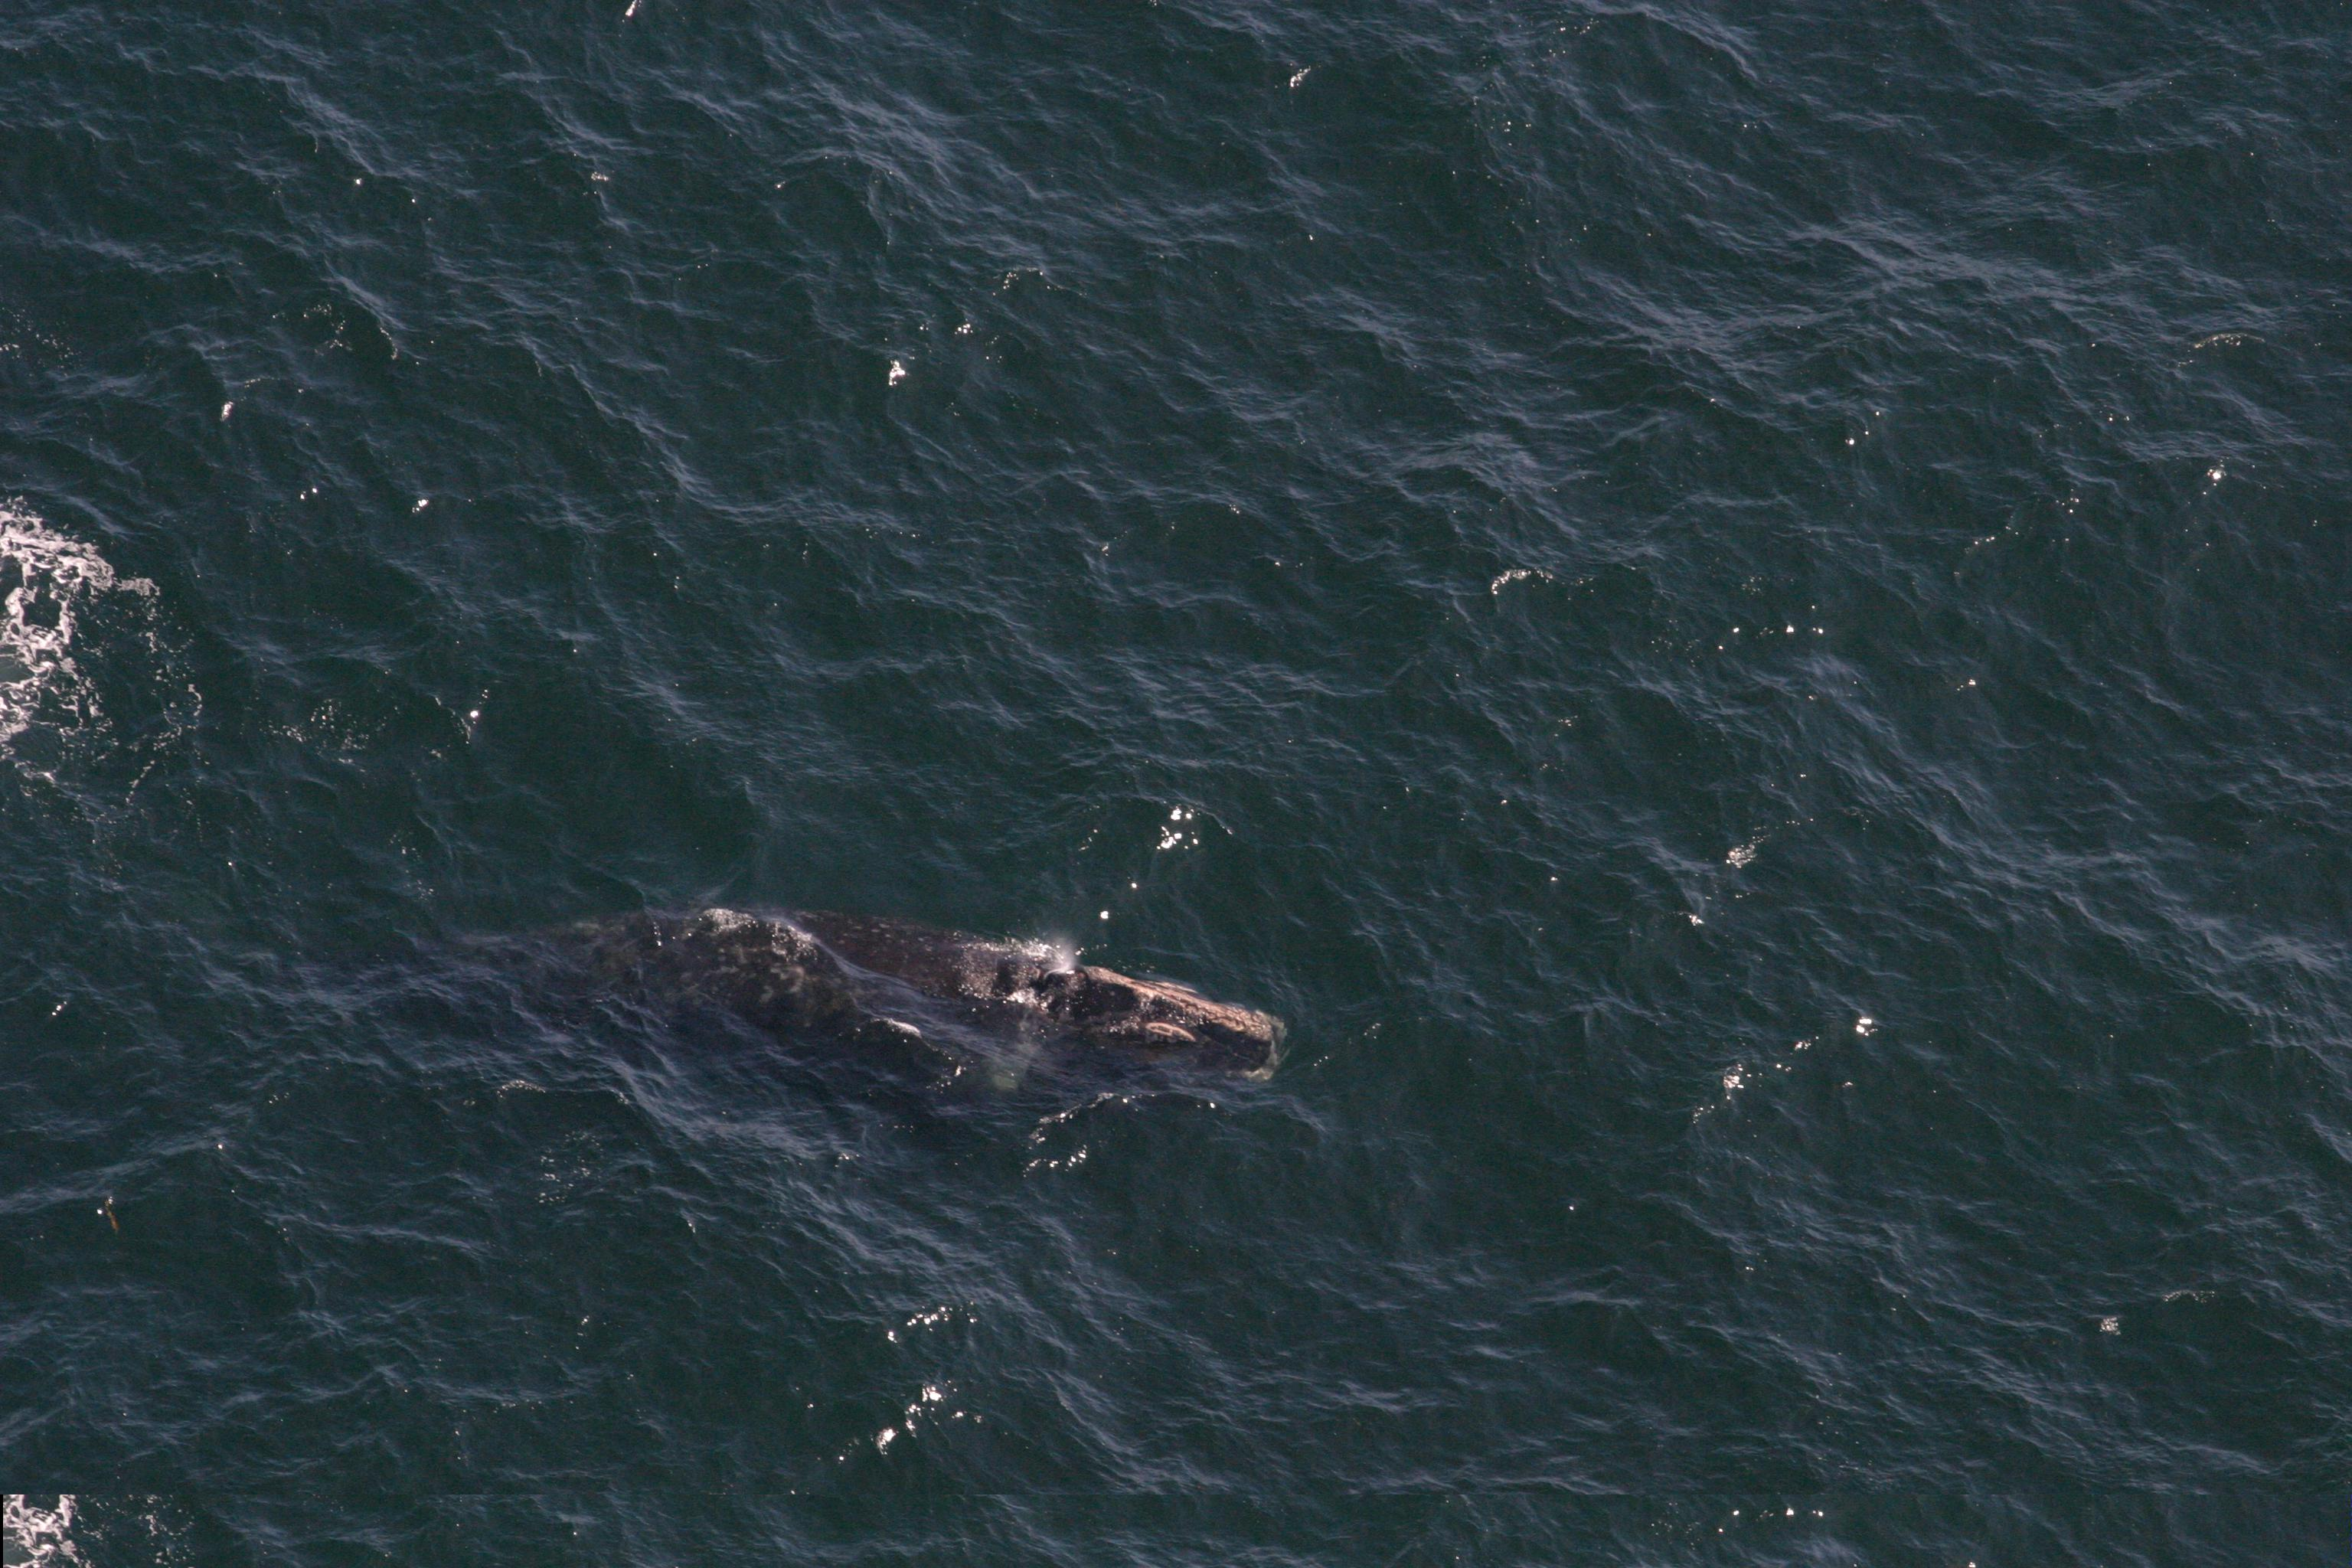
\includegraphics[width=\linewidth]{Images/w_7489.jpg}
	\caption{Example of whale from the dataset}
	\label{fig:whale-example}
\end{figure}

Min: 1
Max: 47
Standard deviation: 

Min: 1
Q1: 5
Median: 9
Mean: 10,17
Q3: 14
Max: 47
SD: 6,8

On average each whale has 10 occurrences within the training data ( )